\section{Motivation}

State channels are an important technique for scaling blockchains.
In a state channel, a fixed set of participants execute a series of state transitions off-chain, in order to determine how a set of assets should be distributed between them.
By allowing participants to execute these transitions off-chain, the state channel removes load from the blockchain, allowing it to support the same level of activity with fewer transactions.

Unlike many other scaling techniques, state channels provide a way to run arbitrary state update protocols, instead of just providing a method for realizing transfers off-chain.

Beyond scaling, state channels bring instant finality to blockchain transactions:
value can be considered to be transferred at the moment when a state channel update is received.
The holder of a fully signed state does not need to wait for the transaction to be mined, safe in the knowledge
that they have the right to claim the assets on-chain at a future point of time of their choosing.

\subsection{Ledger Channels and Virtual Channels}

In their naive form, a group of participants need a new state channel for each application they run and each state channel needs to have a corresponding \textit{state deposit} - a set of assets held in escrow on-chain, to be distributed according to the outcome of the channel.
Each time a state channel is opened, at least one party needs to perform an on-chain transaction to transfer assets into the state deposit, and each time it is closed at least one participant must perform an on-chain transaction to claim their share.
This limits the effectiveness of state channels as a scaling solution, making it only suitable for the case where a large number of transactions are executed between a single group of participants.
We refer to these naive channels as \textbf{direct channels}, as they are supported directly by funds held on the blockchain.

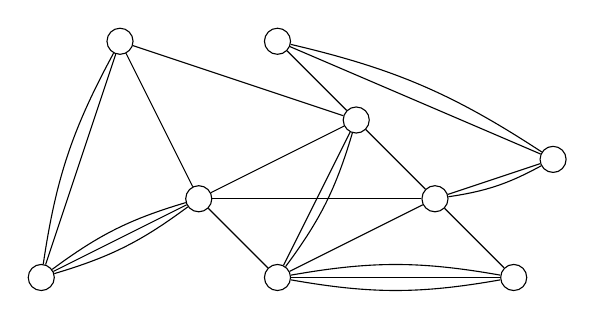
\begin{tikzpicture}
  \begin{scope}[every node/.style={circle, draw}]
    \node (a) at (0,0) {} ;
    \node (b) at (-1,2) {} ;
    \node (c) at (1,-1) {} ;
    \node (d) at (2,1) {} ;
    \node (e) at (1,2) {} ;
    \node (f) at (-2,-1) {} ;
    \node (g) at (3,0) {} ;
    \node (h) at (4,-1) {} ;
    \node (i) at (4.5,0.5) {} ;
  \end{scope}

  \begin{scope}[-]
    \draw (a) to (b);
    \draw (a) to (c);
    \draw (a) to (f);
    \draw (a) to (d);
    \draw (a) to (g);
    \draw (b) to (f);
    \draw (c) to (h);
    \draw (c) to (g);
    \draw (d) to (c);
    \draw (d) to (b);
    \draw (g) to (h);
    \draw (g) to (i);
    \draw (g) to (d);
    \draw (e) to (d);
    \draw (e) to (i);
    % \draw (e) to (a);
    \draw (f) to[bend left=10] (b);
    \draw (f) to[bend left=10] (a);
    \draw (f) to[bend right=10] (a);
    \draw (e) to[bend left=10] (i);
    \draw (g) to[bend right=10] (i);
    \draw (c) to[bend right=10] (d);
    \draw (c) to[bend right=10] (h);
    \draw (c) to[bend left=10] (h);
  \end{scope}
\end{tikzpicture}

- ledger channels 
- one deposit between a pair of participants
- can run multiple applications

- virtual channels
- for example in a hub and spoke model
- participants would connect with one 

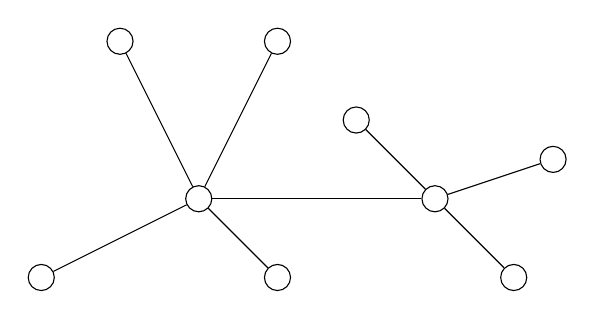
\begin{tikzpicture}
  \begin{scope}[every node/.style={circle, draw}]
    \node (a) at (0,0) {} ;
    \node (b) at (-1,2) {} ;
    \node (c) at (1,-1) {} ;
    \node (d) at (2,1) {} ;
    \node (e) at (1,2) {} ;
    \node (f) at (-2,-1) {} ;
    \node (g) at (3,0) {} ;
    \node (h) at (4,-1) {} ;
    \node (i) at (4.5,0.5) {} ;
  \end{scope}

  \begin{scope}[-]
    \draw (a) to (b);
    \draw (a) to (c);
    \draw (a) to (f);
    \draw (a) to (e);
    \draw (a) to (g);
    \draw (g) to (h);
    \draw (g) to (i);
    \draw (g) to (d);
  \end{scope}
\end{tikzpicture}

- graph of ledger channels with single lines between nodes

- graph of virtual channels with hub + spoke

- image of virtual channels, talking about the agreements


\subsection{Our contribution}

- detailed description of how to build ledger + virtual channels
- the basis for reasoning about the correctness of construction of these channels

- unique:
  - no time limit - instead allowing participants to offload channels
  - n-parties
  - arbitrary applications
